%Master File:lectures.tex


\lesson{Differential Calculus}
\vspace{-1cm}
\begin{center}
  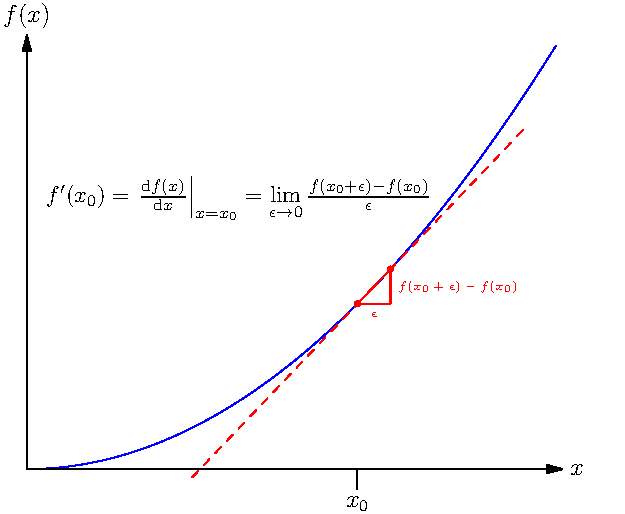
\includegraphics[height=10cm]{derivative-2}
\end{center}
\keywords{Differentiation, product and chain rules, vectors and matrices}
%%%%%%%%%%%%%%%%%%%%%%% Next Slide %%%%%%%%%%%%%%%%%%%%%%%
\renewcommand{\Outline}{%
\begin{slide}
\section[1]{Outline}

\begin{minipage}{10cm}\raggedright
  \begin{enumerate}\squeeze
    \outlineitem{Why Calculus?}{calculus}
    \outlineitem{Differentiation}{differentiation}
    \outlineitem{Vector and Matrix Calculus}{vector}
  \end{enumerate}
\end{minipage}\hfill
\begin{minipage}{12cm}
  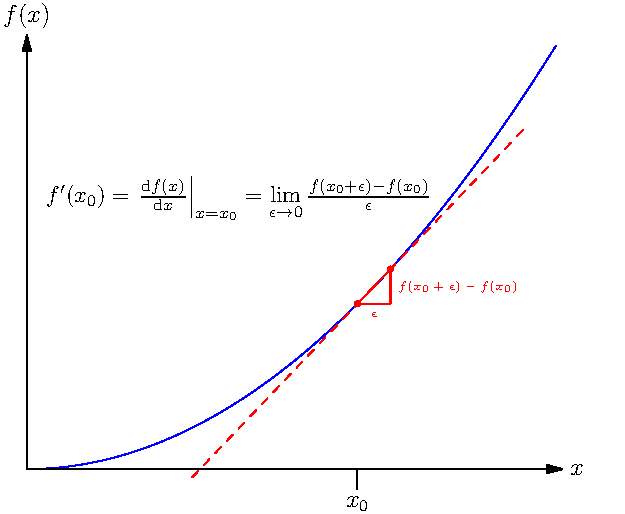
\includegraphics[width=12cm]{derivative-2}
\end{minipage}
\end{slide}
\addtocounter{outlineitem}{1}
}

\newcommand{\bits}{\,\mathrm{bits}}
\setcounter{outlineitem}{1}


%%%%%%%%%%%%%%%%%%%%%%% Next Slide %%%%%%%%%%%%%%%%%%%%%%%
\Outline % Why Calculus
%%%%%%%%%%%%%%%%%%%%%%% Next Slide %%%%%%%%%%%%%%%%%%%%%%%

\begin{slide}
\section{Why Calculus?}

\begin{PauseHighLight}
  \begin{itemize}
  \item Calculus is a fundamental tool of mathematical analysis\pause
  \item In machine learning differentiation is fundamental tool in
    optimisation\pause
  \item Integration is an essential tool in taking expectations over
    continuous distributions\pause
  \item Both differentiation and integration crop up elsewhere\pause
  \item This material will not be examined explicitly\pauseb, but I
    assume elsewhere that you can do calculus\pauseb
  \end{itemize}
\end{PauseHighLight}

\end{slide}

%%%%%%%%%%%%%%%%%%%%%%% Next Slide %%%%%%%%%%%%%%%%%%%%%%%

\begin{slide}
\section{Back to Basics}
  
\begin{PauseHighLight}
  \begin{itemize}
  \item You have all done A-level maths so should be familiar with the
    rules of calculus\pause
  \item But, it is easy to forget the rules and sometimes we use quite
    sophisticated tricks\pause
  \item Although the sophisticated tricks really speed up
    calculations, it pays to be able to understand where these tricks
    come from\pause
  \end{itemize}
\end{PauseHighLight}

\end{slide}

%%%%%%%%%%%%%%%%%%%%%%% Next Slide %%%%%%%%%%%%%%%%%%%%%%%
\Outline % Differentiation
%%%%%%%%%%%%%%%%%%%%%%% Next Slide %%%%%%%%%%%%%%%%%%%%%%%

\begin{slide}
  \section[-1]{Differentiation}

  \pb \pause \pauselevel{=1}
  \begin{center}
    \multipdf[width=0.7\linewidth]{derivative}\pause
  \end{center}

\end{slide}

%%%%%%%%%%%%%%%%%%%%%%% Next Slide %%%%%%%%%%%%%%%%%%%%%%%

\begin{slide}
\section{Polynomials}

\begin{PauseHighLight}
  \begin{itemize}
  \item $f(x)=x^2$
    \begin{align*}
      \frac{\dd x^2}{\dd x} &= \lim_{\epsilon\rightarrow 0}
      \frac{(x+\epsilon)^2 - x^2}{\epsilon}\pause
      =  \lim_{\epsilon\rightarrow 0}
      \frac{(x^2 + 2\,\epsilon\,x + \epsilon^2) -
                              x^2}{\epsilon}\pauseb
                              \\
      &= \lim_{\epsilon\rightarrow 0} 2\,x + \epsilon\pauseb = 2\,x\pauseb
    \end{align*}
  \item $(x+\epsilon)^n =
    (x+\epsilon)(x+\epsilon)\cdots(x+\epsilon)\pauseb = x^n +
    n\,\epsilon\,x^{n-1} + O(\epsilon^2)$\pauseb
     \begin{align*}
      \frac{\dd x^n}{\dd x} &= \lim_{\epsilon\rightarrow 0}
      \frac{(x+\epsilon)^n - x^n}{\epsilon}\pauseb
      =   \lim_{\epsilon\rightarrow 0} n\,x^{n-1} + O(\epsilon)\pauseb = n\,x^{n-1}\pauseb
    \end{align*}
  \end{itemize}
\end{PauseHighLight}

\end{slide}

%%%%%%%%%%%%%%%%%%%%%%% Next Slide %%%%%%%%%%%%%%%%%%%%%%%

\begin{slide}
\section{Linearity of derivatives}
  
\begin{PauseHighLight}
  \begin{itemize}
  \item Note that $f(x+\epsilon) = f(x) + \epsilon\, f'(x) +
    O(\epsilon^2)$ (from the definition of $f'(x)$)\pause
    \begin{align*}
      \frac{\dd \bra{a\,f(x)+b\,g(x)}}{\dd x}
      &=
      \lim_{\epsilon\rightarrow 0}
      \frac{\bra{a\,f(x+\epsilon)+b\,g(x+\epsilon)}-\bra{a\,f(x)+b\,g(x)}}{\epsilon}
      \pause \\
      &=  \lim_{\epsilon\rightarrow 0}
        \frac{a\,\epsilon\, f'(x) +b\,\epsilon\,g'(x) +
        O(\epsilon^2)}{\epsilon}\pauseb \\
      &= a\,f'(x) + b\,g'(x) \pauseb
    \end{align*}
  \item \emph{Differentiation is a linear operation!}\pauseb
  \end{itemize}
\end{PauseHighLight}

\end{slide}

%%%%%%%%%%%%%%%%%%%%%%% Next Slide %%%%%%%%%%%%%%%%%%%%%%%

\begin{slide}
\section[-1]{Linearity in Pictures}

 \pb \pause \pauselevel{=1}
  \begin{center}
    \multipdf[width=0.8\linewidth]{difflinearity}\pause
  \end{center}

\end{slide}

%%%%%%%%%%%%%%%%%%%%%%% Next Slide %%%%%%%%%%%%%%%%%%%%%%%

\begin{slide}
  \section{Product Rule}

\begin{PauseHighLight}
  \begin{itemize}
  \item Recall $f(x+\epsilon) = f(x) + \epsilon\, f'(x) + O(\epsilon^2)$
  \item If $h(x) = f(x)\, g(x)$\pause
    {\small
    \begin{align*}
      h'(x) &= \lim_{\epsilon\rightarrow 0}
      \frac{f(x+\epsilon)\,g(x+\epsilon)-f(x)\,g(x)}{\epsilon}\pauseb \\
      &= \lim_{\epsilon\rightarrow 0} \frac{\bra{f(x) + \epsilon\, f'(x) +
    O(\epsilon^2)} \bra{g(x) + \epsilon\, g'(x) +
              O(\epsilon^2)}-f(x)\,g(x)}{\epsilon}\pauseb \\
      &= \lim_{\epsilon\rightarrow 0} \frac{\epsilon \bra{f'(x)\,g(x) +
        f(x)\,g'(x)}+O(\epsilon^2)}{\epsilon}\pauseb
        = f'(x)\,g(x) + f(x)\,g'(x)\pauseb
    \end{align*}}
  \item This is the \emph{product rule}\pauseb
  \end{itemize}
\end{PauseHighLight}

\end{slide}

%%%%%%%%%%%%%%%%%%%%%%% Next Slide %%%%%%%%%%%%%%%%%%%%%%%

\begin{slide}
\section[-2]{Chain Rule}

\begin{PauseHighLight}
  \begin{itemize}
  \item Recall $f(x+\epsilon) = f(x) + \epsilon\, f'(x) + O(\epsilon^2)$
  \item Let $h(x) = f(g(x))$\pause
  \item Then
    \begin{align*}
      h(x+\epsilon) &= f(g(x+\epsilon)) \pause= f\bra{g(x) + \epsilon\,g'(x) +
                      O(\epsilon^2)}\pauseb\\
      &= f(g(x)) + \epsilon\, g'(x)\, f'(g(x)) + O(\epsilon^2)\pauseb
    \end{align*}
  \item Thus
    \begin{align*}
      h'(x) =  \lim_{\epsilon\rightarrow 0} \frac{h(x+\epsilon)  -
      h(x)}{\epsilon} = g'(x)\, f'(g(x)) \pauseb
    \end{align*}
  \item This is the famous \emph{chain rule}\pauseb. Together with the
    product rule it means you can differentiate almost everything\pauseb
  \end{itemize}
\end{PauseHighLight}

\end{slide}

%%%%%%%%%%%%%%%%%%%%%%% Next Slide %%%%%%%%%%%%%%%%%%%%%%%

\begin{slide}
\section{More on chain rules}

\begin{PauseHighLight}
  \begin{itemize}
  \item We can also write the chain rule as
    \begin{align*}
      \frac{\dd f(g(x))}{\dd x} = \frac{\dd f(g)}{\dd g} \, \frac{\dd
      g(x)}{\dd x}\pause
    \end{align*}
  \item Sometimes this is neater or easier to remember
    \begin{align*}
      \frac{\dd \e{\cos(x^2)}}{\dd x}
      &= \frac{\dd \e{\cos(x^2)}}{\dd \cos(x^2)} \,
        \frac{\dd \cos(x^2)}{\dd x^2} \frac{\dd x^2}{\dd x}\pause\\
      &= \e{\cos(x^2)} \bra{-\sin(x^2)} \, 2\,x\pauseb  \\
      &= -2\, x\, \sin(x^2) \, \e{\cos(x^2)}\pauseb
    \end{align*}
  \end{itemize}
\end{PauseHighLight}

\end{slide}


%%%%%%%%%%%%%%%%%%%%%%% Next Slide %%%%%%%%%%%%%%%%%%%%%%%

\begin{slide}
\section[-2]{Inverse functions}

\begin{PauseHighLight}
  \begin{itemize}
  \item Suppose $g(y) = f^{-1}(y)$ is the inverse of $f(x)$ in the sense that
    $g(f(x)) = f^{-1}(f(x))=x$\pause
  \item Using the chain rule
    \begin{align*}
      \frac{\dd g(f(x))}{\dd x} = f'(x)\, g'(f(x))\pause = 1
    \end{align*}
    since $g(f(x))= x$\pauseb
  \item  So $g'(f(x))= 1/f'(x)$\pause
   \item Writing $y=f(x)$ so that $x=f^{-1}(y) = g(y)$ we find $g'(y)
     = 1/f'(g(y))$ that is
     \begin{align*}
       \frac{\dd g(y)}{\dd y} &= \frac{1}{f'(g(y))}\pause &
       \frac{\dd f^{-1}(y)}{\dd y} &= \frac{1}{f'(f^{-1}(y))}\pauseb                            
     \end{align*}
  \end{itemize}
\end{PauseHighLight}


\end{slide}



%%%%%%%%%%%%%%%%%%%%%%% Next Slide %%%%%%%%%%%%%%%%%%%%%%%

\begin{slide}
  \section{Exponentials}

\begin{PauseHighLight}
  \begin{itemize}
  \item Note that $a^{b+c} = a^b \, a^c$ (that is we multiply $a$
    together $b+c$ times)\pauseb
  \item Now $\e{\epsilon} \approx (1+\epsilon) $\hfil\hfil \raisebox{-2cm}{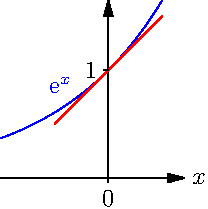
\includegraphics[height=4cm]{expeps}}\pauseb
  \item But $\e{x+\epsilon} = \e{x}\,\e{\epsilon} = \e{x}(1+\epsilon +
    O(\epsilon^2))\pauseb = \e{x} + \epsilon\,\e{x}+ O(\epsilon^2)$\pauseb
    \begin{align*}
      \frac{\dd \e{x}}{\dd x} = \lim_{\epsilon\rightarrow 0}
      \frac{\e{x+\epsilon}-\e{x}}{\epsilon}\pauseb
      =  \lim_{\epsilon\rightarrow 0} \frac{\epsilon\,\e{x} +
      O(\epsilon^2)}{\epsilon} = \e{x}\pauseb
    \end{align*}
  \end{itemize}
\end{PauseHighLight}

\end{slide}

%%%%%%%%%%%%%%%%%%%%%%% Next Slide %%%%%%%%%%%%%%%%%%%%%%%

\begin{slide}
\section[-1]{Functions of Exponentials}

\begin{PauseHighLight}
  \begin{itemize}
  \item What about $f(x)= \e{c\,x}$
    \begin{align*}
      \frac{\dd \e{c\,x}}{\dd x} = \frac{\dd \e{c\,x}}{\dd c\,x} \;
      \frac{\dd c\,x}{\dd x} \pause=   c \, \e{c\,x}\pauseb
    \end{align*}
  \item More generally using the chain rule
    \begin{align*}
       \frac{\dd \e{g(x)}}{\dd x} = g'(x)\,\e{g(x)}\pause
    \end{align*}
  \item Also $a^{b\,c} = (a^b)^c$ (that is we multiply $a$
    together $b\times c$ times)\pauseb
    \begin{align*}
      \frac{\dd a^x}{\dd x} = \frac{\dd (\e{\ln(a)})^x }{\dd x}\pauseb =
      \frac{\dd \e{\ln(a)\, x}}{\dd x}\pauseb = \ln(a)\,  \e{\ln(a)\, x}\pauseb =
      \ln(a)\, a^x\pauseb
    \end{align*}
  \end{itemize}
\end{PauseHighLight}

\end{slide}

%%%%%%%%%%%%%%%%%%%%%%% Next Slide %%%%%%%%%%%%%%%%%%%%%%%

\begin{slide}
\section{Natural Logarithms}

\begin{PauseHighLight}
  \begin{itemize}
  \item The natural logarithm is defined as the inverse of $\e{x}$
    \begin{align*}
      \ln(\e{x}) &= x  & \e{\ln(y)} =y\pause
    \end{align*}
  \item Recall that if $g(y)= f^{-1}(y)$ then $g'(y) =
    1/f'(g(y))$\pause
  \item Consider $g(y)=\ln(y)$ and $f(x)= \e{x}$ (with $f'(x)=\e{x}$)
    \begin{align*}
      \frac{\dd \ln(y)}{\dd y} = \frac{1}{\e{\ln(y)}}\pause = \frac{1}{y}\pauseb
    \end{align*}
   \end{itemize}
\end{PauseHighLight}

\end{slide}

%%%%%%%%%%%%%%%%%%%%%%% Next Slide %%%%%%%%%%%%%%%%%%%%%%%

\begin{slide}
\section[-2]{Exponentials and Logarithms}

\pb
\pause\pauselevel{=1} 
\begin{center}
\multipdf[width=0.9\linewidth]{invExp}\pause  
\end{center}

\end{slide}


%%%%%%%%%%%%%%%%%%%%%%% Next Slide %%%%%%%%%%%%%%%%%%%%%%%
\Outline % Differentiation in High Dimenstions
%%%%%%%%%%%%%%%%%%%%%%% Next Slide %%%%%%%%%%%%%%%%%%%%%%%

\begin{slide}
\section{Derivatives in High Dimensions}

\begin{PauseHighLight}
  \begin{itemize}
  \item When working with functions $f:\mathbb{R}^n \rightarrow
    \mathbb{R}$ in many dimensions then there will typically be
    different derivative in different directions\pause
  \item To compute the derivative in a direction
    $\bm{u} \in \mathbb{R}^n$ (where $\len{\bm{u}}=1$) at a point
    $\bm{x} \in \mathbb{R}^n$ we use
    \begin{align*}
      \partial_{\bm{u}} F(\bm{x}) = \lim_{\epsilon\rightarrow0}\;
      \frac{f(\bm{x}+ \epsilon \bm{u}) - f(\bm{x})}{\epsilon}\pause
    \end{align*}
  \item If $\bm{u} = \bm{\delta}_i = (0,\ldots,0,1,0,\ldots,0)$
    (i.e. $u_i = 1$) then
    \begin{align*}
      \pd{f(\bm{x})}{x_i} = \lim_{\epsilon\rightarrow0}\;
      \frac{f(\bm{x}+ \epsilon \bm{\delta}_i) - f(\bm{x})}{\epsilon}\pause
    \end{align*}
  \end{itemize}
\end{PauseHighLight}

\end{slide}

%%%%%%%%%%%%%%%%%%%%%%% Next Slide %%%%%%%%%%%%%%%%%%%%%%%

\begin{slide}
\section[-2]{Taylor}

\begin{PauseHighLight}
  \begin{itemize}
  \item If we expand $f(\bm{x}+ \epsilon \bm{u})$ to first order in $\epsilon$
    \begin{align*}
      f(\bm{x}+ \epsilon \bm{u})  = f(\bm{x})  + \epsilon \,
      \bm{u}^\tr \bm{g}(\bm{x}) + O(\epsilon^2)
    \end{align*}
    then $g_i(\bm{x}) = \pd{f(\bm{x})}{x_i}$\pause
  \item Recall we defined the vector of first order derivatives of
    $f(\bm{x})$ to be the gradient
  \vspace{-1cm}
    {\small
    \begin{align*}
      \grad f(\bm{x})  =
      \begin{pmatrix}
        \pd{f(\bm{x})}{x_1} \\ \pd{f(\bm{x})}{x_2}  \\ \vdots \\ \pd{f(\bm{x})}{x_n} 
      \end{pmatrix}\pause
    \end{align*}}
  \vspace{-3cm}
  
  \item Thus
     \begin{align*}
      f(\bm{x}+ \epsilon \bm{u})  = f(\bm{x})  + \epsilon \,
      \bm{u}^\tr \grad f(\bm{x})  + O(\epsilon^2)\pause
     \end{align*}
     This is the start of the high-dimensional Taylor expansion\pauseb
  \end{itemize}
\end{PauseHighLight}

\end{slide}

%%%%%%%%%%%%%%%%%%%%%%% Next Slide %%%%%%%%%%%%%%%%%%%%%%%

\begin{slide}
\section{Computing Gradients 1}

\begin{PauseHighLight}
  \begin{itemize}
  \item We can compute the gradient by writing out $f(\bm{x})$
    componentwise and performing the partial derivative with respect
    to $x_i$\pause
    \begin{align*}
      \grad \bm{w}^\tr \mat{M}\, \bm{w}\pause &=
      \begin{pmatrix}
        \pd{\ }{w_1} \\  \pd{\ }{w_2} \\  \pd{\ }{w_3} \\ \vdots
      \end{pmatrix}
      \sum_{i,j} w_i M_{ij} w_j \pauseb =
      \begin{pmatrix}
        \sum_j M_{1j} w_j + \sum_i w_i M_{i1} \\
        \sum_j M_{2j} w_j + \sum_i w_i M_{i2} \\
        \sum_j M_{3j} w_j + \sum_i w_i M_{i3} \\ \vdots
      \end{pmatrix} \pauseb\\
      &= \mat{M}\, \bm{w} + \mat{M}^\tr\, \bm{w}\pauseb
    \end{align*}
  \item It is tedious to compute these things component-wise, but when
    you need to understand what is going on then go back to the basics\pauseb
  \end{itemize}
\end{PauseHighLight}
  

\end{slide}



%%%%%%%%%%%%%%%%%%%%%%% Next Slide %%%%%%%%%%%%%%%%%%%%%%%

\begin{slide}
\section{Computing Gradients 2}

\begin{PauseHighLight}
  \begin{itemize}
  \item A slicker way is just to expand $f(\bm{x}+ \epsilon
    \bm{u})$\pause
  \item Consider $f(\bm{x}) = \bm{x}^\tr \mat{M}\,\bm{x} +
    \bm{a}^\tr\bm{x}$
    \begin{align*}
      f(\bm{x}+ \epsilon \bm{u}) &= (\bm{x}+ \epsilon \bm{u})^\tr
      \mat{M}\, (\bm{x}+ \epsilon \bm{u})  +    \bm{a}^\tr(\bm{x}+
      \epsilon \bm{u}) \pause\\
      &= f(\bm{x}) + \epsilon\bra{ \bm{u}^\tr\mat{M}\, \bm{x} +
        \bm{x}^\tr\mat{M}\, \bm{u} + \bm{a}^\tr\bm{u}} +O(\epsilon^2)  \pauseb\\
      &= f(\bm{x}) + \epsilon\, \bm{u}^\tr \bra{\mat{M}\, \bm{x}+
        \mat{M}^\tr\, \bm{x} + \bm{a} }+O(\epsilon^2) 
    \end{align*}
    using $\bm{x}^\tr\mat{M}\, \bm{u}  = \bm{u}^\tr\mat{M}^\tr\,
    \bm{x}$ and $\bm{a}^\tr\bm{u} = \bm{u}^\tr\bm{a}$\pauseb
  \item But $
      f(\bm{x}+ \epsilon \bm{u})  = f(\bm{x})  + \epsilon \,
      \bm{u}^\tr \grad f(\bm{x})  + O(\epsilon^2)$ so
    \begin{align*}
      \grad f(\bm{x}) = \mat{M}\, \bm{x}+
        \mat{M}^\tr\, \bm{x} + \bm{a} \pauseb
    \end{align*}
  \end{itemize}
\end{PauseHighLight}

\end{slide}

%%%%%%%%%%%%%%%%%%%%%%% Next Slide %%%%%%%%%%%%%%%%%%%%%%%

\begin{slide}
\section{Differentiating Matrices}

\begin{PauseHighLight}
  \begin{itemize}
  \item Often we have loss functions with respect to a matrix
    $\mat{W}$, e.g.
    \begin{align*}
      L(\mat{W}) = (\bm{a}^\tr \mat{W} \bm{b} - c)^2\pause
    \end{align*}
  \item We might want to find the minimum with respect to
    $\mat{W}$\pause
  \item This occurs at a point $\mat{W}^*$ where $L(\mat{W})$ does not
    increase as we change $\mat{W}$ in any way\pause
  \item That is, we seek a $\mat{W}^*$ such that, for any matrices $\mat{U}$
    \begin{align*}
      L(\mat{W}^*+\epsilon \mat{U}) - L(\mat{W}^*) = O(\epsilon^2)\pause
    \end{align*}
  \end{itemize}
\end{PauseHighLight}

\end{slide}

%%%%%%%%%%%%%%%%%%%%%%% Next Slide %%%%%%%%%%%%%%%%%%%%%%%

\begin{slide}
\section[-2]{Generalised Gradient}

\begin{PauseHighLight}
  \begin{itemize}
  \item We can generalise the idea of gradient to matrices
    \begin{align*}
      \pd{L(\mat{W})}{\mat{W}} =
      \begin{pmatrix}
        \pd{L(\mat{W})}{W_{11}} & \pd{L(\mat{W})}{W_{12}} & \cdots & \pd{L(\mat{W})}{W_{1m}} \\ 
        \pd{L(\mat{W})}{W_{21}} & \pd{L(\mat{W})}{W_{22}} & \cdots & \pd{L(\mat{W})}{W_{2m}} \\ 
        \vdots & \vdots & \ddots & \vdots \\
        \pd{L(\mat{W})}{W_{n1}} & \pd{L(\mat{W})}{W_{n2}} & \cdots & \pd{L(\mat{W})}{W_{nm}} \\ 
      \end{pmatrix}\pause
    \end{align*}
  \item From an identical argument we used for vectors
    \begin{align*}
      L(\mat{W}+\epsilon \mat{U}) = L(\mat{W}) + \epsilon\,
      \mathrm{tr}\,  \mat{U}^\tr \,  \pd{L(\mat{W})}{\mat{W}} + O(\epsilon^2)\pause
    \end{align*}
    where
    \begin{align*}
      \mathrm{tr}\, \mat{U}^\tr  \mat{G} = \sum_{i} \left[   \mat{U}^\tr
      \mat{G}\right]_{ii} = \sum_{ij} U_{ji} G_{ji} = \sum_{ij} U_{ij} G_{ij} = \langle \mat{U},
      \mat{G} \rangle\pause
    \end{align*}
  \end{itemize}
\end{PauseHighLight}

\end{slide}

%%%%%%%%%%%%%%%%%%%%%%% Next Slide %%%%%%%%%%%%%%%%%%%%%%%

\begin{slide}
\section[-1]{Example}

\begin{PauseHighLight}
  \begin{itemize}
  \item Suppose
    \begin{align*}
      L(\mat{W}) = \bra{\bm{a}^\tr \mat{W} \bm{b} - c}^2\pause
    \end{align*}
    then
    \begin{align*}
      L(\mat{W}+\epsilon \mat{U})
      &= \bra{\bm{a}^\tr (\mat{W}+\epsilon\mat{U}) \bm{b} - c}^2 \pause
        = \bra{\bm{a}^\tr \mat{W} \bm{b} + \epsilon\,
        \bm{a}^\tr \mat{U} \bm{b}  - c}^2 \pauseb \\
      &= L(\mat{W})  + 2\,\epsilon \bra{\bm{a}^\tr \mat{W} \bm{b} -
        c}\bra{ \bm{a}^\tr \mat{U} \bm{b}} + O(\epsilon^2)\pauseb
    \end{align*}
  \item Now
    \begin{align*}
      \bm{a}^\tr \mat{U} \bm{b} = \sum_{ij} a_i\, U_{ij}\, b_j \pauseb=\sum_{ij}
      U_{ji}\, a_j \, b_i \pauseb =
      \mathrm{tr}\, \mat{U}^\tr \bm{a} \bm{b}^\tr\pauseb
    \end{align*}
    Thus $\pd{L(\mat{W})}{\mat{W}} = 2\,\bra{\bm{a}^\tr \mat{W} \bm{b} -
        c}\bm{a} \bm{b}^\tr$\pauseb
  \end{itemize}
\end{PauseHighLight}

\end{slide}

%%%%%%%%%%%%%%%%%%%%%%% Next Slide %%%%%%%%%%%%%%%%%%%%%%%

\begin{slide}
\section[-2]{Traces}

\begin{PauseHighLight}\squeeze
  \begin{itemize}
  \item The trace of a matrix is the sum of its diagonal elements
    \begin{align*}
      \mathrm{tr}\, \mat{A} = \mathrm{tr} \, \mat{A}^\tr = \sum_i A_{ii}\pause
    \end{align*}
  \item Clearly $\mathrm{tr} \, c\, \mat{A} = c\, \mathrm{tr}\,
    \mat{A}$\pause
  \item Also $\mathrm{tr} \, (\mat{A} + \mat{B}) = \mathrm{tr} \mat{A}
    + \mathrm{tr} \mat{B}$ \pause
  \item We note that
    \begin{align*}
      \mathrm{tr}\, \mat{A} \,\mat{B} = \sum_{i,j} A_{ij} B_{ji} =
      \sum_{i,j} B_{ij} A_{ji} =  \mathrm{tr} \mat{B} \, \mat{A}\pause
    \end{align*}
  \item It follows that
        \begin{align*}
      \mathrm{tr}\, \mat{A} \,\mat{B}\,\mat{C}\, \mat{D} =
      \mathrm{tr}\, \mat{D}\, \mat{A} \,\mat{B}\,\mat{C}\pause =
      \mathrm{tr}\, \mat{C} \,\mat{D}\,\mat{A}\mat{B}\pauseb =
      \mathrm{tr}\, \mat{B} \,\mat{C}\,\mat{D}\mat{A}\pauseb
    \end{align*}
  \end{itemize}
\end{PauseHighLight}

\end{slide}

%%%%%%%%%%%%%%%%%%%%%%% Next Slide %%%%%%%%%%%%%%%%%%%%%%%

\begin{slide}
\section[-2]{Quick Matrix Differentiation}

\begin{PauseHighLight}
  \begin{itemize}
  \item Let
    \begin{align*}
      \partial_{\mat{U}} f(\mat{X}) = \lim_{\epsilon\rightarrow0}
      \frac{f(\mat{X}+\epsilon \mat{U}) - f(\mat{X})}{\epsilon}\pause
      = \mathrm{tr}\,  \mat{U}^\tr \,  \pd{f(\mat{X})}{\mat{X}}\pauseb
    \end{align*}
  \item E.g.
    \begin{align*}
      \partial_{\mat{U}} \mathrm{tr} \mat{A} \, \mat{X} \mat{B}
      &=  \lim_{\epsilon\rightarrow0} \frac{1}{\epsilon}  \mathrm{tr}
        \mat{A} \, \bra{\strut \mat{X} + \epsilon \mat{U}} \mat{B} -
        \mathrm{tr} \mat{A} \, \mat{X} \mat{B} \\
      &= \mathrm{tr}\; \mat{A} \, \mat{U} \, \mat{B}\pause
      = \mathrm{tr} \;\mat{B}^\tr \, \mat{U}^\tr \, \mat{A}^\tr\pauseb
      = \mathrm{tr} \; \mat{U}^\tr \mat{A}^\tr\, \mat{B}^\tr \pauseb
    \end{align*}
    thus
    \begin{align*}
      \pd{ \mathrm{tr} \mat{A} \, \mat{X} \mat{B} }{\mat{X}} =  \mat{A}^\tr\, \mat{B}^\tr \pauseb
    \end{align*}
  \end{itemize}
\end{PauseHighLight}

\end{slide}

%%%%%%%%%%%%%%%%%%%%%%% Next Slide %%%%%%%%%%%%%%%%%%%%%%%

\begin{slide}
  \section[-2]{Log Determinants}

\begin{PauseHighLight}
  \begin{itemize}
  \item We often come across logarithms of determinants of matrices,
    $\logg{|\mat{M}|}$\pause 
  \item For GP we want to choose $\mat{K}$ to maximise the marginal likelihood,
    $\logg{|\mat{K}+\sigma^2\mat{I}|}$\pause 
  \item To find the derivative of $\logg{|\mat{X}|}$ we consider
    \begin{align*}
      \logg{|\mat{X}+\epsilon\,\mat{U}|}
      &= \logg{|\mat{X}(\mat{I} + \epsilon\,\mat{X}^{-1}\mat{U})|}
        \pause\\
      &= \logg{|\mat{X}| \, |\mat{I} + \epsilon\,\mat{X}^{-1}\mat{U}|}
        \pauseb\\
        &= \logg{|\mat{X}|} + \logg{|\mat{I} + \epsilon\,\mat{X}^{-1}\mat{U}|}\pauseb
    \end{align*}{\small
    \begin{itemize}\squeeze
    \item Using $|\mat{A}\mat{B}| = |\mat{A}| \, |\mat{B}|$
      \pauselevel{=4, build}\pause
    \item Using $\log(a\,b) = \log(a) + \log(b)$  \pauselevel{=5, build}\pause
    \end{itemize}}
  \end{itemize}
\end{PauseHighLight}

\end{slide}

%%%%%%%%%%%%%%%%%%%%%%% Next Slide %%%%%%%%%%%%%%%%%%%%%%%

\begin{slide}
\section[-2]{Determinants}

\pb \pause
{\small
\begin{align*}
  |\mat{I}+\epsilon\,\mat{M}| &=
  \begin{vmatrix}
    1+\epsilon\, M_{11} & \epsilon\, M_{12}\\
    \epsilon\, M_{21} & 1+\epsilon\, M_{22}
  \end{vmatrix}\pauseh
                        = (1+\epsilon\, M_{11})\,(1+\epsilon\, M_{22}) -
                        \epsilon^2\, M_{21}\,M_{12}\pause \\
  &= 1 + \epsilon \bra{M_{11} + M_{22}} + O(\epsilon^2)\pause
\end{align*}}
\begin{center}
  \multipdf[width=0.7\linewidth]{diffdet}\pause
\end{center}


\end{slide}

%%%%%%%%%%%%%%%%%%%%%%% Next Slide %%%%%%%%%%%%%%%%%%%%%%%

\begin{slide}
\section[-2]{Putting it Together}

\begin{PauseHighLight}
  \begin{itemize}
  \item Recall
    \begin{align*}
      \logg{|\mat{X}+\epsilon\,\mat{U}|} - \logg{|\mat{X}|}
      &= \logg{|\mat{I} + \epsilon\,\mat{X}^{-1}\mat{U}|}\pause \\
      &= \logg{1 + \epsilon \, \mathrm{tr}\; \mat{X}^{-1}\mat{U}+
        O(\epsilon)^2}\pauseb\\
        &=  \epsilon \, \mathrm{tr}\; \mat{X}^{-1}\mat{U}+
        O(\epsilon)^2\pauseb\\
        &= \epsilon \, \mathrm{tr}\; \mat{U}^\tr \bra{\mat{X}^{-1}}^\tr+ O(\epsilon)\pauseb
    \end{align*}
    using $\log(1+x) = x + \tfrac{x^2}{2} +
    \cdots$\pauselevel{=3, build, highlight}\pause \pauselevel{=5}
    \item Thus $\partial_{\mat{U}} \logg{|\mat{X}|} = \mathrm{tr}\;
      \mat{U}^\tr \bra{\mat{X}^{-1}}^\tr$\pauseb
    \item Or
      \begin{align*}
        \frac{\partial \logg{|\mat{X}|}}{\partial \mat{X}} =  \bra{\mat{X}^{-1}}^\tr\pauseb
      \end{align*}

  \end{itemize}
\end{PauseHighLight}

\end{slide}


%%%%%%%%%%%%%%%%%%%%%%% Next Slide %%%%%%%%%%%%%%%%%%%%%%%

\begin{slide}
\section{Summary}
  
\begin{PauseHighLight}
  \begin{itemize}
  \item With care you can differentiate most expressions\pause
  \item The chain and product rule are incredibly powerful tools\pause
  \item We can generalise differentiation to vectors and
    matrices\pause
  \item There are a number of surprisingly useful results\pause: see
    \emph{The Matrix Cookbook}\pauseb
  \item Next stop: integration\pauseb
  \end{itemize}
\end{PauseHighLight}

\end{slide}

